\section{Raspberry Pi - Google Assistant}

\subsection{Projekt fizyczny}

Na podstawie schematu (dostępnego w poprzednim rozdziale) został zbudowany prototyp urządzenia pełniącego rolę asystenta.

\begin{center}
\adjustbox{valign=t}{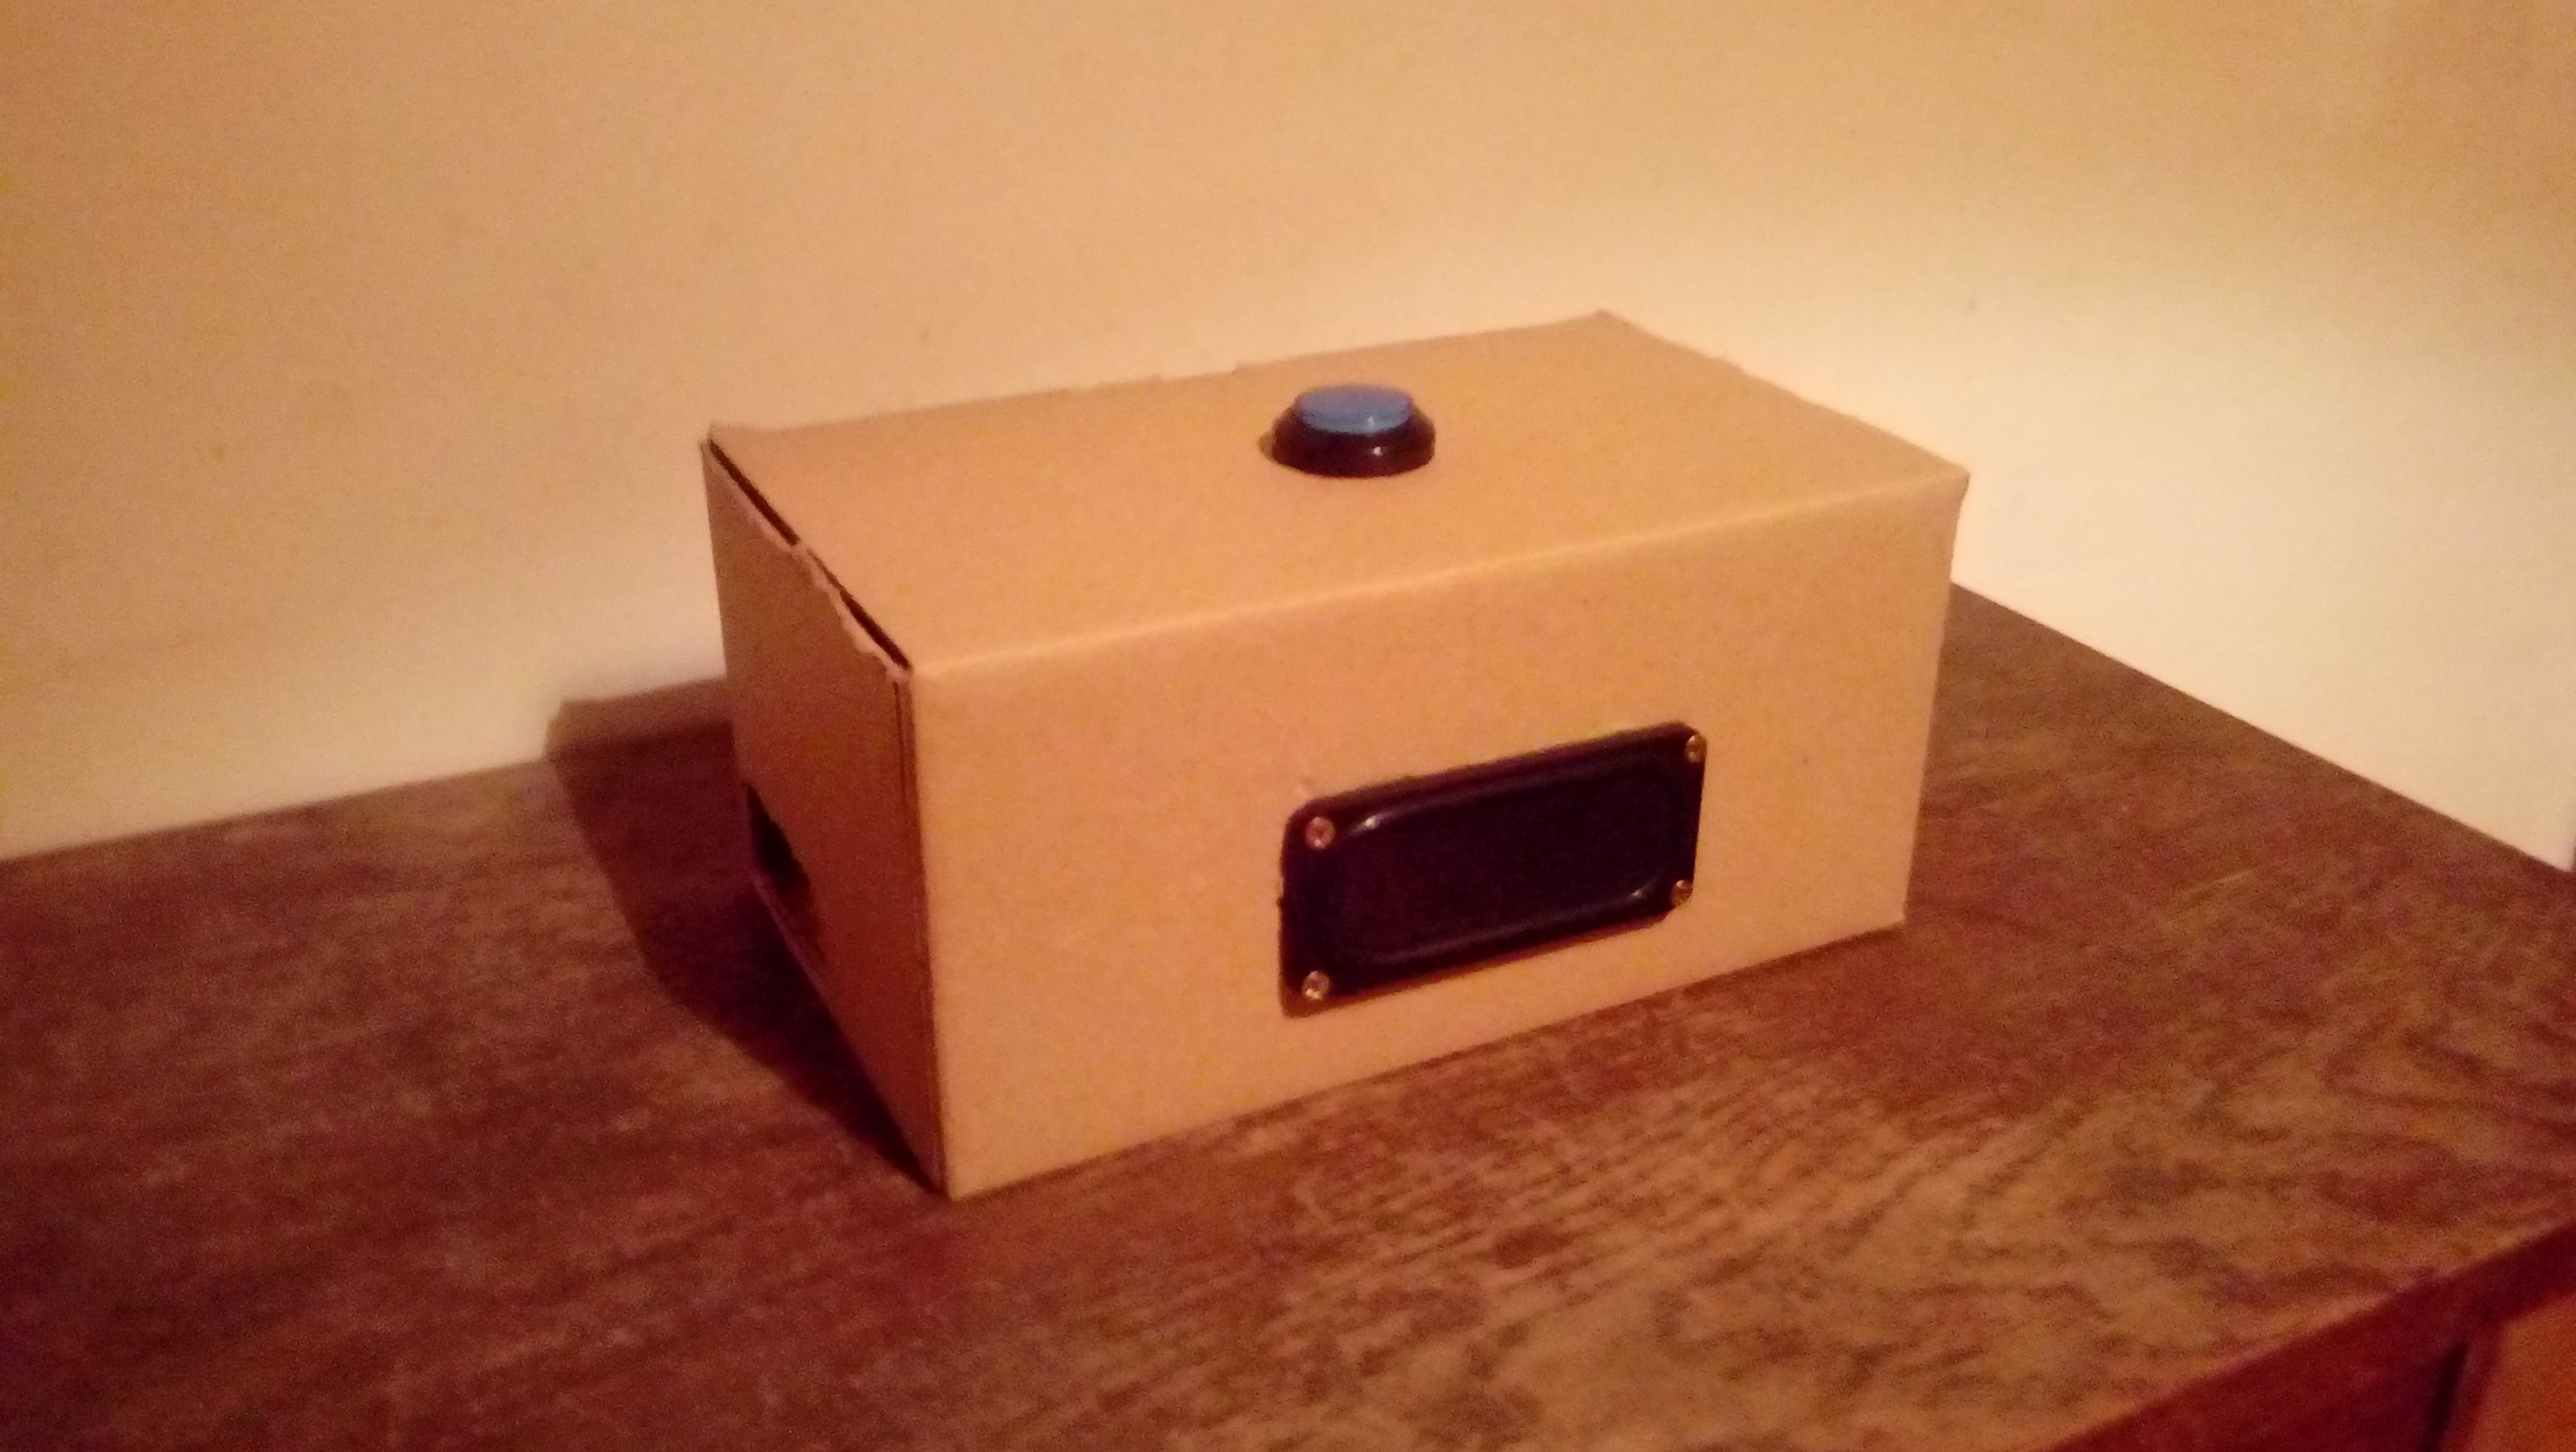
\includegraphics[width=10cm]{out.jpg}}
\end{center}
	
\begin{center}
\adjustbox{valign=t}{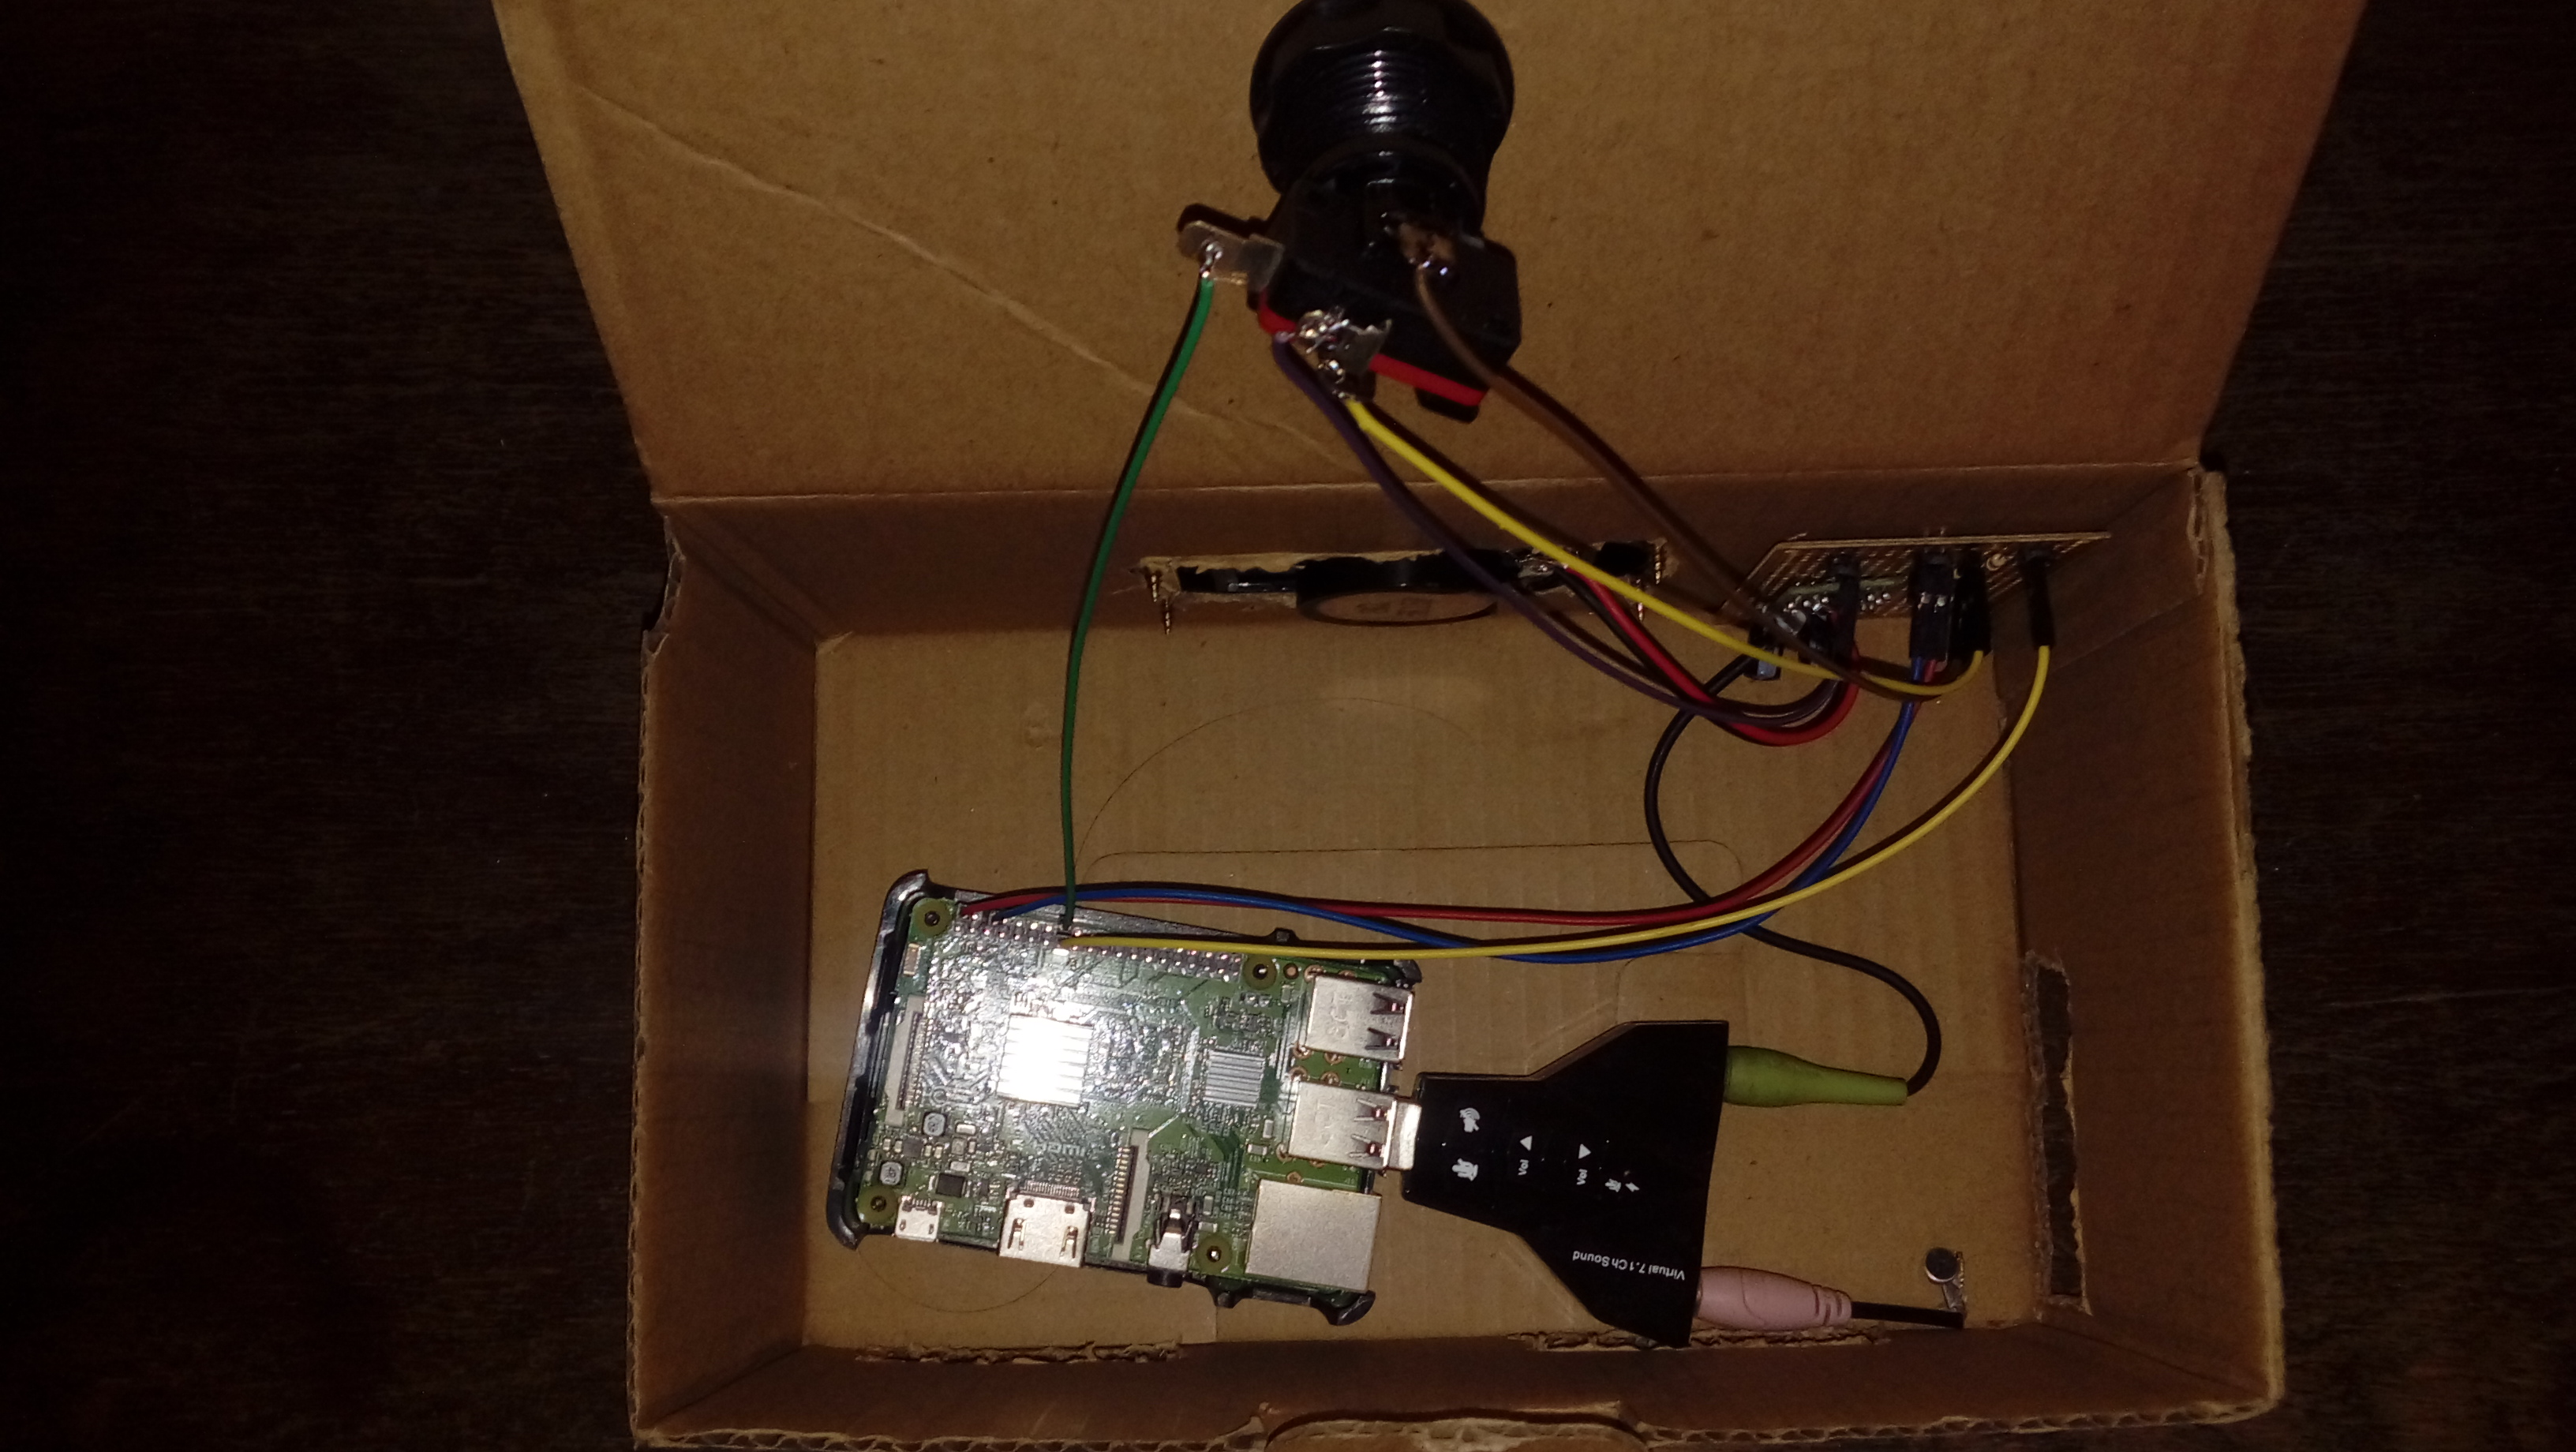
\includegraphics[width=10cm]{in.jpg}}
\end{center}

\subsection{Instalacja Google Assistant}

Podstawowa konfiguracja Google Assistant jest bardzo dobrze opisana na stronie \url{https://developers.google.com/assistant/sdk/overview} (zakładka ,,Python'').

\subsection{Opis pliku wejściowego}

Zakładając projekt z wykorzystujący Google Assistant SDK dostajemy skrypt realizujący podstawową funkcjonalność asystenta:


\begin{lstlisting}[language=Python]
#!/usr/bin/env python

# Copyright (C) 2017 Google Inc.
#
# Licensed under the Apache License, Version 2.0 (the 'License');
# you may not use this file except in compliance with the License.
# You may obtain a copy of the License at
#
#     http://www.apache.org/licenses/LICENSE-2.0
#
# Unless required by applicable law or agreed to in writing, software
# distributed under the License is distributed on an 'AS IS' BASIS,
# WITHOUT WARRANTIES OR CONDITIONS OF ANY KIND, either express or implied.
# See the License for the specific language governing permissions and
# limitations under the License.


from __future__ import print_function

import argparse
import os.path
import json

import google.oauth2.credentials

from google.assistant.library import Assistant
from google.assistant.library.event import EventType
from google.assistant.library.file_helpers import existing_file


def process_event(event):
    '''Pretty prints events.
    Prints all events that occur with two spaces between each new
    conversation and a single space between turns of a conversation.
    Args:
        event(event.Event): The current event to process.
    '''
    if event.type == EventType.ON_CONVERSATION_TURN_STARTED:
        print()

    print(event)

    if (event.type == EventType.ON_CONVERSATION_TURN_FINISHED and
            event.args and not event.args['with_follow_on_turn']):
        print()


def main():
    parser = argparse.ArgumentParser(
        formatter_class=argparse.RawTextHelpFormatter)
    parser.add_argument('--credentials', type=existing_file,
                        metavar='OAUTH2_CREDENTIALS_FILE',
                        default=os.path.join(
                            os.path.expanduser('~/.config'),
                            'google-oauthlib-tool',
                            'credentials.json'
                        ),
                        help='Path to store and read OAuth2 credentials')
    args = parser.parse_args()
    with open(args.credentials, 'r') as f:
        credentials = google.oauth2.credentials.Credentials(token=None,
                                                            **json.load(f))

    with Assistant(credentials) as assistant:
        for event in assistant.start():
            process_event(event)


if __name__ == '__main__':
    main()
    
\end{lstlisting}

Powyższy kod tworzy obiekt asystenta (wykorzystując w tym procesie dane uwierzytelniające),
po czym w pętli zaczyna przetwarzanie zdarzeń (przykładem zdarzenia jest początek konwersacji wywoływany słowami ,,Hey Google'').
Zmieniając implementację metody process\_event możemy wpływać na zachowanie asystenta.


\begin{lstlisting}[language=Python]
def process_event(cp, event, assistant):
    '''Pretty prints events.
    Prints all events that occur with two spaces between each new
    conversation and a single space between turns of a conversation.
    Args:
        event(event.Event): The current event to process.
    '''
    if event.type == EventType.ON_CONVERSATION_TURN_STARTED:
        print()
        gpio.output(22, True)

    print(event)
    
    if event.type == EventType.ON_RECOGNIZING_SPEECH_FINISHED:
        try:
            if cp.read_command(event.args['text']):
                assistant.stop_conversation()
        except ValueError as e:
            print(e)
            
    if (event.type == EventType.ON_CONVERSATION_TURN_FINISHED and
            event.args and not event.args['with_follow_on_turn']):
        print()
        gpio.output(22, False)
\end{lstlisting}

Powyższy kod przedstawia zmodyfikowaną wersję metody process\_event. Najważniejszym elementem jest przechwycenie zdarzenia ,,ON RECOGNIZING SPEECH FINISHED'', w którym można znaleźć nasze słowa zamienione na tekst (ang. Speech To Text). Dzięki temu, odpowiednio przetwarzając zdarzenie, możemy zaimplementować własne reakcje systemu. W tym celu stworzyliśmy klasę (opisaną dokładniej w dalszej części dokumentu) ,,CommandProcessor'' (cp). Przyjmuje ona treść naszych słów i szuka odpowiedniej komendy do wywołania - w przypadku znalezienia takowej, ,,rozmowa'' z asystentem jest przerywana (nie usłyszymy odpowiedzi od sztucznej inteligencji). W powyższej metodzie dopisaliśmy również reakcje na zdarzenia ,,ON CONVERSATION TURN STARTED'' i ,,ON CONVERSATION TURN FINISHED'' jest to odpowiednio zapalanie i gaszenie diody.

\subsection{Własne komendy}

W celu umożliwienia stworzenia własnych komend powstał skrypt ,,commands\_processor.py'':



\begin{lstlisting}[language=Python]

from inspect import signature
import RPi.GPIO as gpio
import time
import subprocess
from subprocess import CalledProcessError, check_output
import _thread
import os

#additional functions
def is_process_alive(process_name):
    try:
        check_output(["pgrep", process_name])
        output = 0
    except subprocess.CalledProcessError as er:
        output = er.returncode
        
    if output == 0:
        return True
    else:
        return False
        
        
def play_sound(filename):
    os.system("aplay sounds/"+filename)

##########



#custom commands:

def print_hello(text):
    print("hello")
    
    
def print_bye(text):
    print("bye")
    
def print_text(text):
	print(text)
	
def play_yt(text):
    
    if is_process_alive("vlc"):
        return
        
    play_sound("im_on_it.wav")
    
    playshell = subprocess.Popen(["/usr/local/bin/mpsyt", ""],
		stdin=subprocess.PIPE, stdout=subprocess.PIPE)
    
    playshell.stdin.write(bytes('/' + text + '\n1\n', 'utf-8'))
    playshell.stdin.flush()
    
    gpio.setmode(gpio.BCM)
    gpio.setup(23, gpio.IN, pull_up_down=gpio.PUD_UP)
    
    print("STARTING VLC...")
    while(not is_process_alive("vlc")):
        time.sleep(1)
        
    print("MUSIC IS PLAYING")    
    while(gpio.input(23) and is_process_alive("vlc")):
        time.sleep(1)
        
    subprocess.Popen(["/usr/bin/pkill", "vlc"], stdin=subprocess.PIPE)
    playshell.kill()
	
##################
	

class CommandProcessor(object):
	
    commands = [
    ("hello", print_hello),
    ("bye", print_bye),
    ("print", print_text),
    ("play", play_yt)
    ]
    
	
    def read_command(self, text):
        try:
            command = next(x for x in self.commands if text.startswith(x[0]))
        except StopIteration as err:
            return False
        
        text = text.replace(command[0], "", 1)
        text = text.strip()
        method = command[1]
           
        sig = signature(method)
        length = len(sig.parameters)
        if (length == 0):
            return _thread.start_new_thread(method, ())
        elif (length == 1):
            _thread.start_new_thread(method, (text,))
        else:
            raise ValueError("EXCEPTION: Trying to call a function
			      with more than one parameter") 
        
        
return True


\end{lstlisting} 

Klasa ,,CommandProcessor'' została wspomniana w poprzednim podrozdziale - przetwarza ona komendy użytkownika decydując o tym, czy były one przeznaczone dla 
asystenta, czy nie. Zmienna ,,commands'' jest mapą słów kluczowych w komendach
na funkcje, które w ramach danej komendy mają być wywołane. Metoda ,,read\_command'' sprawdza czy pierwsze słowa wypowiedzi użytkownika 
znajdują się w zmiennej ,,commands''. Jeżeli tak, to w osobnym wątku wywoływana jest odpowiednia funkcja (przykłady funkcji można znaleźć wyżej w kodzie)
i zwracana jest wartość True, jeżeli nie to zwracana jest wartość False.

\section{ESP8266}

\subsection{Projekt fizyczny}

Na podstawie schematu (dostępnego w poprzednim rozdziale) został zbudowany prototyp czujników z nadajnikiem zbierający dane o stanie zapełnienia skrzynki.

\subsection{Pierwsze użycie płytki i konfiguracja IDE}

Przed pierwszym użyciem płytki jest zalecana zaktualizowanie jej firmware'u. Dobra instrukcja wykonania tego znajduje się na stronie \url{http://hobbyspace.pl/nodemcu-jak-wgrac-firmware/}.

Do oprogramowania płytki zostało wykorzystane Arduino IDE (v.1.8.5). W celu uzyskania możliwości współpracy z wcześniej wspomnianym IDE konieczne było dodanie dodatkowego adresu URL dla menadżera płytek w zakładce preferencje. Oto wymagany tam link \url{http://arduino.esp8266.com/stable/package_esp8266com_index.json}
Po uzupełnieniu źródłem w Narzędzia->Płytka->Menedżer płytek możliwe stało się odnalezienie "ESP8266 Comunity" instalujemy najnowszą wersję (w naszym przypadku 2.3.0). Po tak przygotowanym IDE możliwe był przystąpienie do pracy.

\subsection{Opis działania programu}

Do oprogramowania płytki został przygotowany poniższy program.

\begin{lstlisting} [language=C++]
#include <ESP8266WiFi.h>
#include <ESP8266HTTPClient.h>

const char* ssid = "*****";  // type your ssid
const char* password = "*****";    // type your password
WiFiClient client;

int IRledPin = 4;                     // Dioda IR nadawcz
int TSOPPin = 5;                      // Dioda TSOP odbiorcza

//Start setup
void setup() {
	pinMode(TSOPPin, INPUT);
	pinMode(IRledPin, OUTPUT);
	digitalWrite(IRledPin, LOW);
	WiFiConnect();
}

//Main loop
void loop() {
	measurement();
	ESP.deepSleep(30e6); // 30e6 is 30 microseconds
}

//////
//IR//
//////

// Measurement IR
void measurement()
{
	digitalWrite(IRledPin, HIGH);
	int resault = pulseIn(TSOPPin,LOW,10000000);  //waiting 10 seconds for IR signal
	digitalWrite(IRledPin, LOW);
	reaction(resault);
}

// Reaction box measurement
void reaction(int resault){
	if(resault == 0){
		SendGET("0.0.0.0.500");
	}
	else{
		SendGET("0.0.0.0.501");
	}
}

////////
//WiFi//
////////

// Connect to WiFi network
void WiFiConnect() {
	WiFi.mode(WIFI_AP_STA);
	WiFi.begin(ssid, password);
	while (WiFi.status() != WL_CONNECTED) {
		delay(500);
	}
}

// Send GET request to URL
void SendGET(String URL)
{
	HTTPClient http;
	
	http.begin(URL);  //Specify request destination
	http.GET();       //Send the request (returning code 
	http.end();
}
\end{lstlisting}

Opisując kolejno w głównej pętli programu \textit{loop} posiadamy dwie funkcje, pierwsza z nich to funkcja własna odpowiadająca za pomiar oraz systemową ESP.deepSleep(time). Ta właśnie funkcja korzysta z wspomnianego w poprzednim rozdziale połączenia pinów GPIO16 oraz RST, pozwalając uśpić 
płytkę na określony w jej parametrze czas, umożliwiając w ten sposób oszczędzenie baterii. Natomiast funkcja \textit{measurement} odpala nam diodę IR, przez 10s nasłuchuje na czujniku czy odbiera sygnał IR. Wynik tego pomiaru jest przekazywany funkcji \textit{reactrion}, która w zależności od parametru wysyła na nasz serwer zapytanie GET albo z parametrem mówiącym o posiadaniu poczty lub też nie.
